% 原分章PDF第1—15页，止于3.1.4节标题之前；原印刷页173—187。
\chapter{可穿戴计算与函数值性状的遗传分析}
\label{ch:wearable-functional-traits}

低成本、无创、无线的可穿戴生物传感器（wearable biosensor）正在迅速发展。这类传感器推动了移动健康（mobile health，mHealth）技术的发展，可以持续监测患者、运动员、早产儿、儿童、精神疾病患者、需要长期照护者、老年人，以及交通不便、远离卫生和医疗服务地区的人群（Ajami and Teimouri 2015）。可穿戴生物传感器使人们能够离开传统医院环境，远程采集数据以追踪身体活动、测量心电图（electrocardiogram，ECG），并记录电信号与光电容积脉搏波（photoplethysmogram，PPG）（Sun et al. 2016）。它们可以实时检测个体健康状态的变化，甚至连续测量个体的分子生理指标，包括代谢物和电解质，从而监测体内正在发生的过程（Gao et al. 2016）。可穿戴计算（wearable computing）有望给卫生保健和疾病管理带来根本变化。

实时采集临床表型和生理表型，是可穿戴生物传感器的一项基本特征。换言之，这类传感器采集的数据呈曲线或函数形式。基于传统生物传感器的疾病预测、检测，以及数量性状的遗传研究，已经得到广泛应用，相关技术也发展充分；相比之下，基于时程数据（time course data）的疾病预测、检测，以及函数值性状的数量遗传分析，发展仍相对不足（Hansen et al. 2011）。越来越多的证据表明，标准多元统计分析往往不适用于函数型数据。函数模型和动态模型可用于疾病分类与函数值性状的遗传研究。本章首先讨论三类可穿戴生物传感器数据分类方法：函数主成分分析、常微分方程和深度学习。随后，建立并分析响应变量与预测变量均为函数的函数型线性模型（functional linear model with functional response and functional predictors，FLMFF），利用下一代测序（next-generation sequencing，NGS）数据开展函数值性状的数量遗传分析。最后讨论函数值性状的基因—基因交互作用模型。

\section{可穿戴生物传感器数据的分类}
\subsection{引言}

可穿戴生物传感器可以连续测量与健康有关的生理指标，包括心电图、心震图（SCG）、血氧饱和度、心率、皮肤温度、血压和身体活动（Li et al. 2017）。这些实时测量呈现为曲线或函数。图3.1给出了心电图的 QRS 波群（QRS complex）。心电信号是一种时变信号，反映了引起心肌纤维收缩、继而舒张的离子电流。QRS 波群通过其组成波形，即 P 波、QRS 波和 T 波的形状变化，承载有关心脏电功能的信息。Q、R、S 三个字母表示一个心动周期的三个主要阶段（Ravier et al. 2007）。QRS 波群被视为心电图中最显著的波形，其形态、幅值和持续时间为心搏的生物过程提供了有价值的信息。

患者上呼吸道阻塞时，体内氧浓度会下降。血氧饱和度在生物学上与睡眠呼吸暂停有关（Varvarigou et al. 2011），一些睡眠呼吸暂停研究也使用血氧饱和度信息。血氧饱和度信号通常按秒测量。图3.2展示了一条典型的整夜氧浓度曲线，共包含35\,280次测量。可穿戴生物传感器采集的这些时程生理表型数据，提供了人体健康状况的重要信息，可以用于疾病监测与诊断。

\begin{figure}[htbp]
\centering
\begin{tikzpicture}[x=1cm,y=1cm]
\node[anchor=south west,inner sep=0] at (0,0) {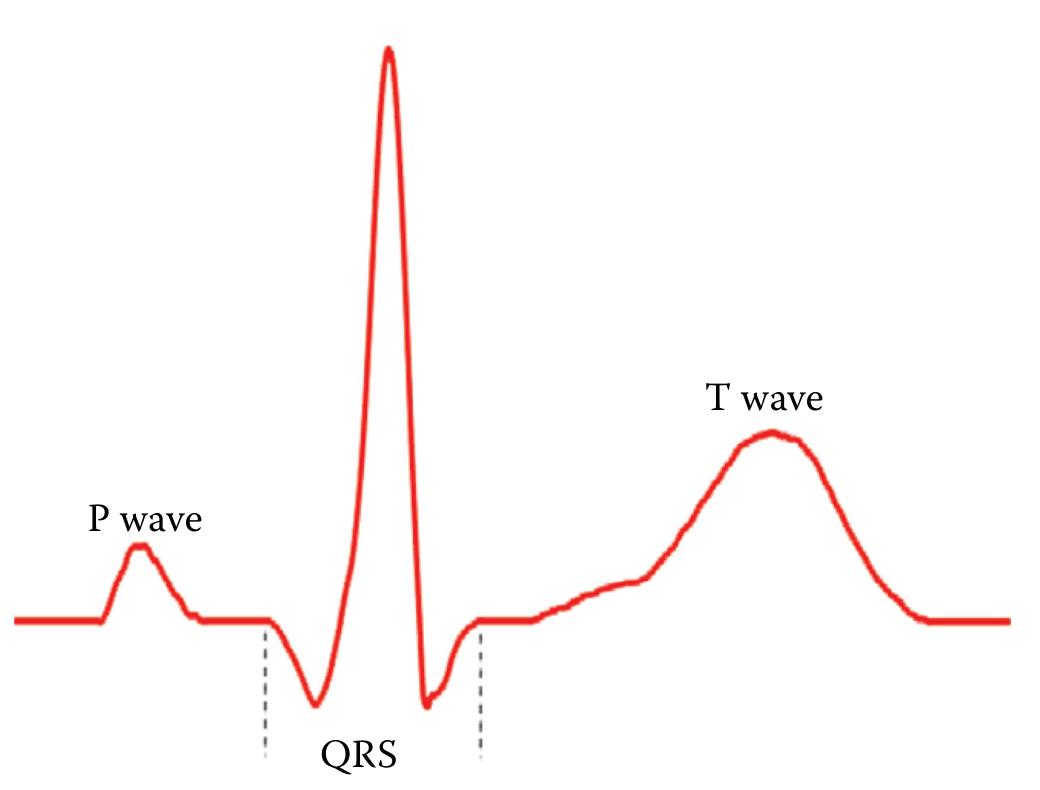
\includegraphics[width=10.0cm]{figures/ch03_fig01_data.png}};
\fill[white] (6.7448,3.5357) rectangle (7.9501,3.9684);
\node[font=\scriptsize,rotate=0,inner sep=0] at (7.3474,3.7521) {T 波};
\fill[white] (0.8109,2.3687) rectangle (1.9771,2.8014);
\node[font=\scriptsize,rotate=0,inner sep=0] at (1.3940,2.5850) {P 波};
\end{tikzpicture}
\origfig{1}{QRS 波群示例。}
\label{fig:ch03-01}
\end{figure}

\begin{figure}[htbp]
\centering
\begin{tikzpicture}[x=1cm,y=1cm]
\node[anchor=south west,inner sep=0] at (0,0) {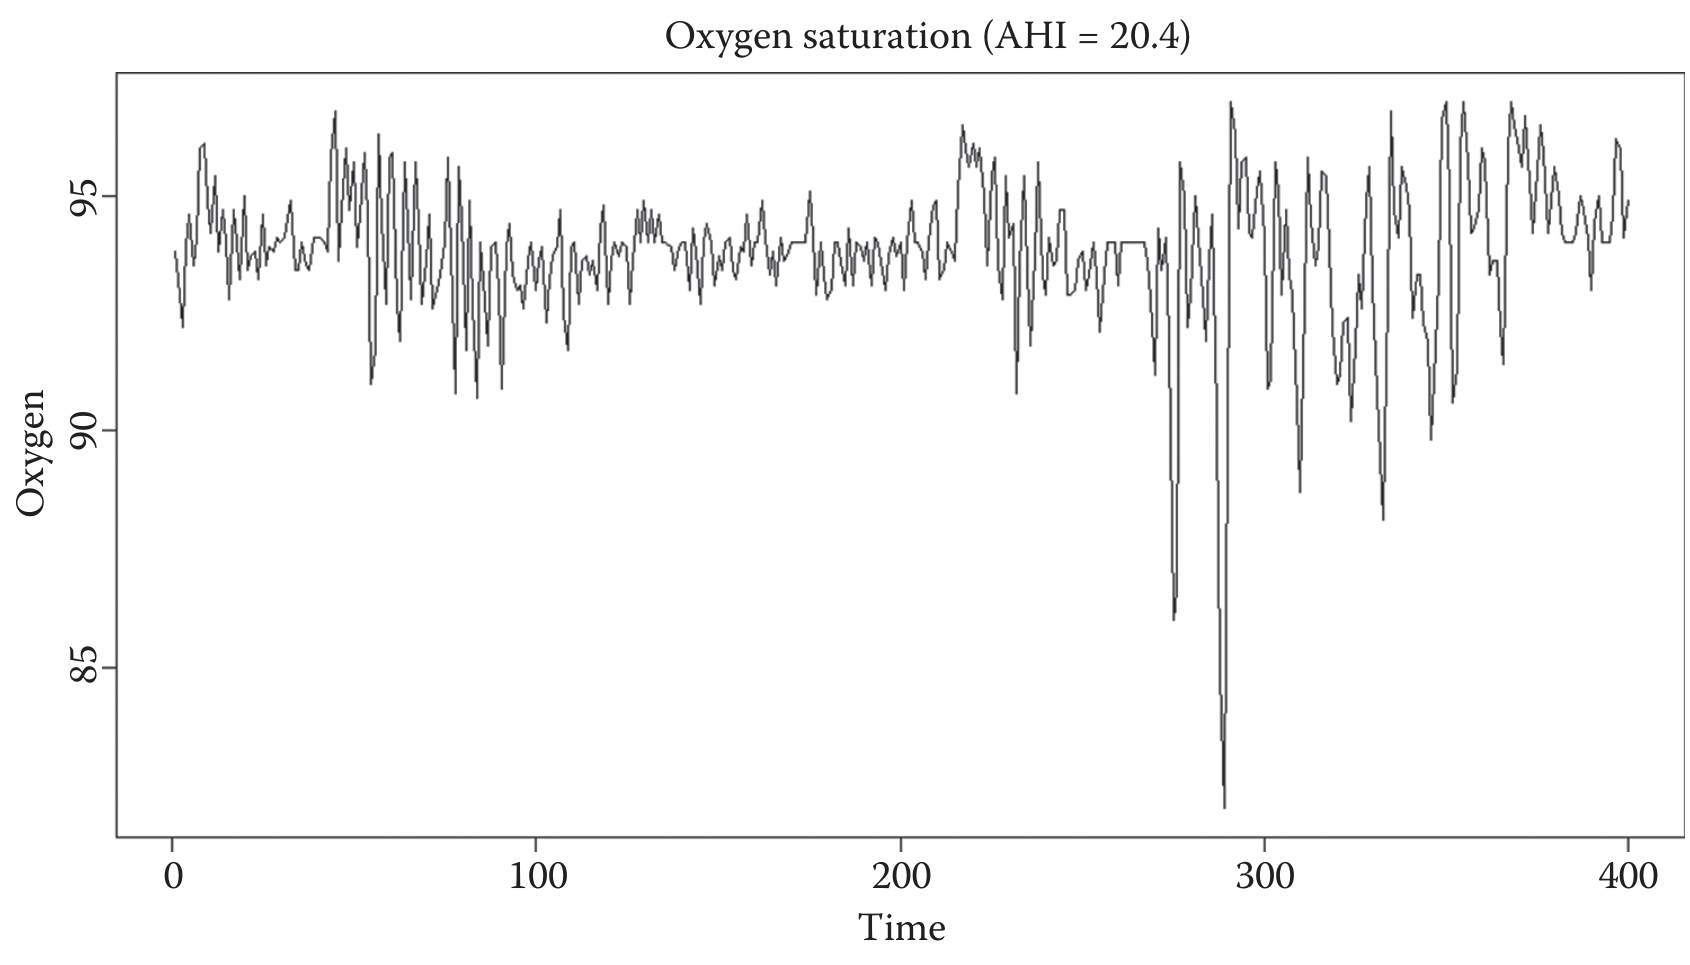
\includegraphics[width=13.8cm]{figures/ch03_fig02_data.png}};
\fill[white] (5.4000,7.3848) rectangle (9.7588,7.7523);
\node[font=\scriptsize,rotate=0,inner sep=0] at (7.5794,7.5686) {血氧饱和度（AHI = 20.4）};
\fill[white] (0.0830,3.6278) rectangle (0.4586,4.7217);
\node[font=\scriptsize,rotate=90,inner sep=0] at (0.2708,4.1747) {血氧};
\fill[white] (6.9743,0.1014) rectangle (7.7523,0.4689);
\node[font=\scriptsize,rotate=0,inner sep=0] at (7.3633,0.2852) {时间};
\end{tikzpicture}
\origfig{2}{血液中的氧浓度。}
\label{fig:ch03-02}
\end{figure}

\FloatBarrier

\subsection{用于可穿戴生物传感器时程数据分类的函数型数据分析}

函数型数据的一个基本特征是维数无限，并且具有高度相关性，这使时程数据的分类变得困难。越来越多的证据表明，标准多元统计分析往往不适用于函数型数据。成功分类时程数据的关键，在于降低数据维数。一种常见做法是选取有限维基，将函数曲线投影到这些基上。所得基展开系数就构成数据的有限维表示。因此，广泛使用的函数型数据统计分类方法包括两个步骤。

第一步，将函数型数据投影到基函数或特征函数张成的有限维空间（Luo et al. 2013；Ramsay and Silverman 2005）。

令 $\phi_j(t)$ 表示一组正交基函数，包括 Fourier 函数、特征函数或函数主成分函数。每个函数均可写成这些基函数的线性组合：
\begin{equation}
x_i(t)=\sum_{j=1}^{\infty}\xi_{ij}\phi_j(t),
\tag{3.1}
\end{equation}
展开系数 $\xi_{ij}$ 估计为
\begin{equation}
\xi_{ij}=\int_Tx_i(t)\phi_j(t)\,dt.
\tag{3.2}
\end{equation}

第二步，使用各种特征选择方法，包括充分降维，以及各种多元数据分类方法，包括线性判别分析（linear discriminant analysis，LDA）、逻辑回归和支持向量机，对展开系数进行分类。

为更有效地利用函数相依信息、突出数据的某些特征，并提高分类准确率，通常需要对函数型数据作不同变换。一般先对数据进行中心化和归一化。其中最重要的一类变换是求导。随后，将原始函数曲线及其各阶导数的线性组合投影到基函数或特征函数上（Alonso et al. 2012）。将动态信息，即导数信息，纳入特征，可以捕捉函数型数据的相依特征，进而改善分类效果。

\subsection{利用微分方程提取动态过程特征并分类时程数据}

将函数导数纳入特征，虽然有望提高分类准确率，但会显著增加特征数量。我们希望在利用动态信息对函数曲线分类时，不增加特征数。对于心电数据中的 QRS 波群等连续变化过程，可以用微分方程描述其动态，并将方程参数作为特征，以达到这一目的。微分方程是描述物理、化学及生物过程中动态系统的有力工具，应用十分广泛。微分方程中的参数刻画真实动态过程的基本行为，并与可用数据相一致。只需少量参数，就可以捕捉系统的基本动态特征。因此，本节讨论如何使用描述动态过程的微分方程参数，对时程数据进行分类。

\subsubsection{用于动态系统建模的常参数与时变参数微分方程}

假设 $x(t)$ 为动态系统的一个状态变量，该系统可以用下列常参数二阶常微分方程（ordinary differential equation，ODE）描述：
\begin{equation}
L(x(t))=\frac{d^2x(t)}{dt^2}
 +w_1\frac{dx(t)}{dt}+w_0x(t)=0,
\tag{3.3}
\end{equation}
或者用时变参数二阶微分方程描述：
\begin{equation}
L(x(t))=\frac{d^2x(t)}{dt^2}
 +w_1(t)\frac{dx(t)}{dt}+w_0(t)x(t)=0.
\tag{3.4}
\end{equation}
其中，$w_1$（或 $w_1(t)$）与 $w_0$（或 $w_0(t)$）是 ODE 的权重系数或参数。状态 $x(t)$ 是隐藏的，其观测值 $y(t)$ 通常含有测量误差：
\begin{equation}
y(t)=x(t)+e(t),
\tag{3.5}
\end{equation}
其中，$e(t)$ 为时刻 $t$ 的测量误差。

\subsubsection{用于微分方程参数估计的主微分分析}

可以通过主微分分析（principal differential analysis）获得 ODE 参数的估计量（Poyton et al. 2006）。参数估计的目的，是确定适当的参数取值，使预测响应值与实测数据之间的误差尽可能小。求解描述动态系统的 ODE，即可获得预测响应值。求解 ODE 的一种方法，是先将函数 $x(t)$ 按基函数展开。令 $x_i(t)$ 为第 $i$ 个样本在时刻 $t$ 的状态变量，满足 ODE (3.3) 或 (3.4)，$y_i(t)$ 为其观测值，$i=1,\ldots,n$。于是
\begin{equation}
x_i(t)=\sum_{j=1}^Kc_{ij}\phi_j(t)=C_i^T\phi(t),
\tag{3.6}
\end{equation}
其中 $C_i=[c_{i1},\ldots,c_{iK}]^T$，
$\phi(t)=[\phi_1(t),\ldots,\phi_K(t)]^T$。
类似地，参数 $w_1(t)$ 与 $w_0(t)$ 可展开为
\begin{equation}
\begin{aligned}
w_1(t)&=\sum_{j=1}^Kh_{1j}\phi_j(t)=h_1^T\phi(t),\\
w_0(t)&=\sum_{j=1}^Kh_{0j}\phi_j(t)=h_0^T\phi(t),
\end{aligned}
\tag{3.7}
\end{equation}
其中
\[
h_1=\begin{bmatrix}h_{11}\\\vdots\\h_{1K}\end{bmatrix},
\qquad
h_0=\begin{bmatrix}h_{01}\\\vdots\\h_{0K}\end{bmatrix}.
\]
令
\[
\begin{aligned}
\psi(t)
&=\frac{d^2\phi}{dt^2}
 +\frac{d\phi}{dt}\phi^T(t)h_1+\phi(t)\phi^T(t)h_0\\
&=\frac{d^2\phi}{dt^2}+G(t)h,
\end{aligned}
\]
以及
\[
J_{\phi h}=\int_T\psi(t)\psi^T(t)\,dt,
\]
其中
\[
G(t)=\begin{bmatrix}
\dfrac{d\phi}{dt}\phi^T(t)&\phi(t)\phi^T(t)
\end{bmatrix},
\qquad
h=\begin{bmatrix}h_1\\h_0\end{bmatrix}.
\]
微分算子为 $L(x_i(t))=C_i^T\psi(t)$。惩罚项定义为
\begin{equation}
\lambda\int_TL(x_i(t))L^T(x_i(t))\,dt
=\lambda C_i^TJ_{\phi h}C_i.
\tag{3.8}
\end{equation}
通过最小化以下目标函数，可以根据观测数据 $y(t)$ 估计状态函数 $x(t)$。目标函数由观测值与状态值之间的误差平方和及惩罚项组成：
\begin{equation}
\begin{aligned}
&\sum_{i=1}^n\left\{
\sum_{j=1}^T[y_i(t_j)-x_i(t_j)]^2
 +\lambda\int_TL(x_i(t))L^T(x_i(t))\,dt\right\}\\
&\qquad=\sum_{i=1}^n\left\{
\sum_{j=1}^T[y_i(t_j)-\phi^T(t_j)C_i]^2
 +\lambda C_i^TJ_{\phi h}C_i\right\}.
\end{aligned}
\tag{3.9}
\end{equation}
令
\[
Y_i=\begin{bmatrix}y_i(t_1)\\\vdots\\y_i(t_T)\end{bmatrix},
\quad
\widetilde\phi=\begin{bmatrix}\phi^T(t_1)\\\vdots\\\phi^T(t_T)\end{bmatrix},
\quad
Y=\begin{bmatrix}Y_1\\\vdots\\Y_n\end{bmatrix},
\]
\[
\Phi=
\begin{bmatrix}
\widetilde\phi&0&\cdots&0\\
\vdots&\vdots&\ddots&0\\
0&0&\cdots&\widetilde\phi
\end{bmatrix},
\quad
J=\begin{bmatrix}
J_{\phi h}&0&\cdots&0\\
0&J_{\phi h}&\cdots&0\\
\vdots&\vdots&\ddots&\vdots\\
0&0&\cdots&J_{\phi h}
\end{bmatrix},
\quad
C=\begin{bmatrix}C_1\\\vdots\\C_n\end{bmatrix}.
\]
于是，问题 (3.9) 可化为
\begin{equation}
\min_C\quad (Y-\Phi C)^T(Y-\Phi C)+\lambda C^TJC.
\tag{3.10}
\end{equation}
展开系数的最小二乘估计量为
\begin{equation}
C=(\Phi^T\Phi+\lambda J)^{-1}\Phi^TY.
\tag{3.11}
\end{equation}

接着估计 ODE 的参数。可以通过最小化以下最小二乘目标函数来估计：
\begin{equation}
\min_h\quad \mathrm{SSE}_p=\int_TL^T(X(t))L(X(t))\,dt,
\tag{3.12}
\end{equation}
其中 $L(X(t))=[L(x_1(t)),\ldots,L(x_n(t))]^T$。由于 $L(x_i(t))=C_i^T\psi(t)$，可以用估计的展开系数表示 $L(X(t))$：
\[
L(X(t))=\widehat C\Psi(t).
\]
因此，问题 (3.3) 可化为
\begin{equation}
\min_h\quad
\mathrm{SSE}_p=\int_T\psi^T(t)\widehat C^T\widehat C\psi(t)\,dt,
\tag{3.13}
\end{equation}
其中矩阵 $\widehat C$ 已经估计，因此在极小化问题 (3.13) 中保持不变。将 $\mathrm{SSE}_p$ 的偏导数置为零：
\begin{equation}
\frac{\partial\mathrm{SSE}_p}{\partial h}
=\int_TG^T(t)\widehat C^T\widehat C
\left[\frac{d^2\phi(t)}{dt^2}+G(t)h\right]dt=0.
\tag{3.14}
\end{equation}
由式 (3.14) 解出 $h$，得到
\begin{equation}
h=-\left[\int_TG^T(t)\widehat C^T\widehat CG(t)\,dt\right]^{-1}
\int_TG^T(t)\widehat C^T\widehat C\frac{d^2\phi}{dt^2}\,dt.
\tag{3.15}
\end{equation}
综上，交替进行以下迭代：固定 ODE 参数，由式 (3.11) 确定展开系数；固定展开系数，由式 (3.15) 估计 ODE 参数，直至收敛。

\subsubsection{QRS 波群实例}
\bookdeepheading{paragraph}{3.1.3.3.1}{ODE 对数据的拟合准确性}

自动心电分析广泛用于心搏分类。它可以监测心脏活动，以及时发现心脏异常，并诊断心律失常。心搏也常用 QRS 波群的形状来表示。Q、R、S 三个字母表示一个心动周期的三个主要阶段（Ravier et al. 2007）。我们将提出的方法用于估计式 (3.4) 和式 (3.5) 的参数，对 QRS 波群建模。首先评价 B 样条（B-spline）对 QRS 波群中信号 $x(t)$ 的拟合效果。数据来自 MIT-BIH 心律失常数据库，其中包含48段双通道动态心电信号（MLII 导联和 V5 导联），每段时长半小时。这里仅使用47名受试者的 MLII 导联。心电信号经过0.1—100\,Hz带通滤波，每个通道以360\,Hz采样，在10\,mV范围内采用3位分辨率（\url{http://www.physionet.org/}）。每条记录由两名或以上心脏病专家独立标注；对分歧进行协商后，形成数据库中每次心搏的计算机可读参考标注。每条记录都有对应的标注文件，提供 QRS 位置、心搏类别等参考信息，分别用于提取 QRS 片段和各次心搏的真实标签。

心电数据由皮肤电极测量和记录，容易受到工频干扰、肌肉收缩、电极移动以及肌电活动等多种噪声污染。为去除不必要的噪声并提高信噪比，对心电波形施加5—12\,Hz带通滤波（低频带和高频带滤波），以消除基线漂移与工频干扰。滤波后的心电信号用于动态模型拟合。图3.3和图3.4分别针对正常与异常 QRS 波群，绘出了观测信号、采用均匀结点间距0.012秒的三次 B 样条拟合曲线，以及常参数和时变参数二阶 ODE 的解轨迹。平滑过程每次迭代中的调节参数均由交叉验证选择。两图均表明，无论正常还是异常波群，三次 B 样条与时变参数二阶 ODE 都能够很好地逼近观测信号。然而，常参数二阶 ODE 的解轨迹无法很好地逼近观测信号，只能得到与观测曲线相似的形状。

\begin{figure}[htbp]
\centering
\begin{tikzpicture}[x=1cm,y=1cm]
\node[anchor=south west,inner sep=0] at (0,0) {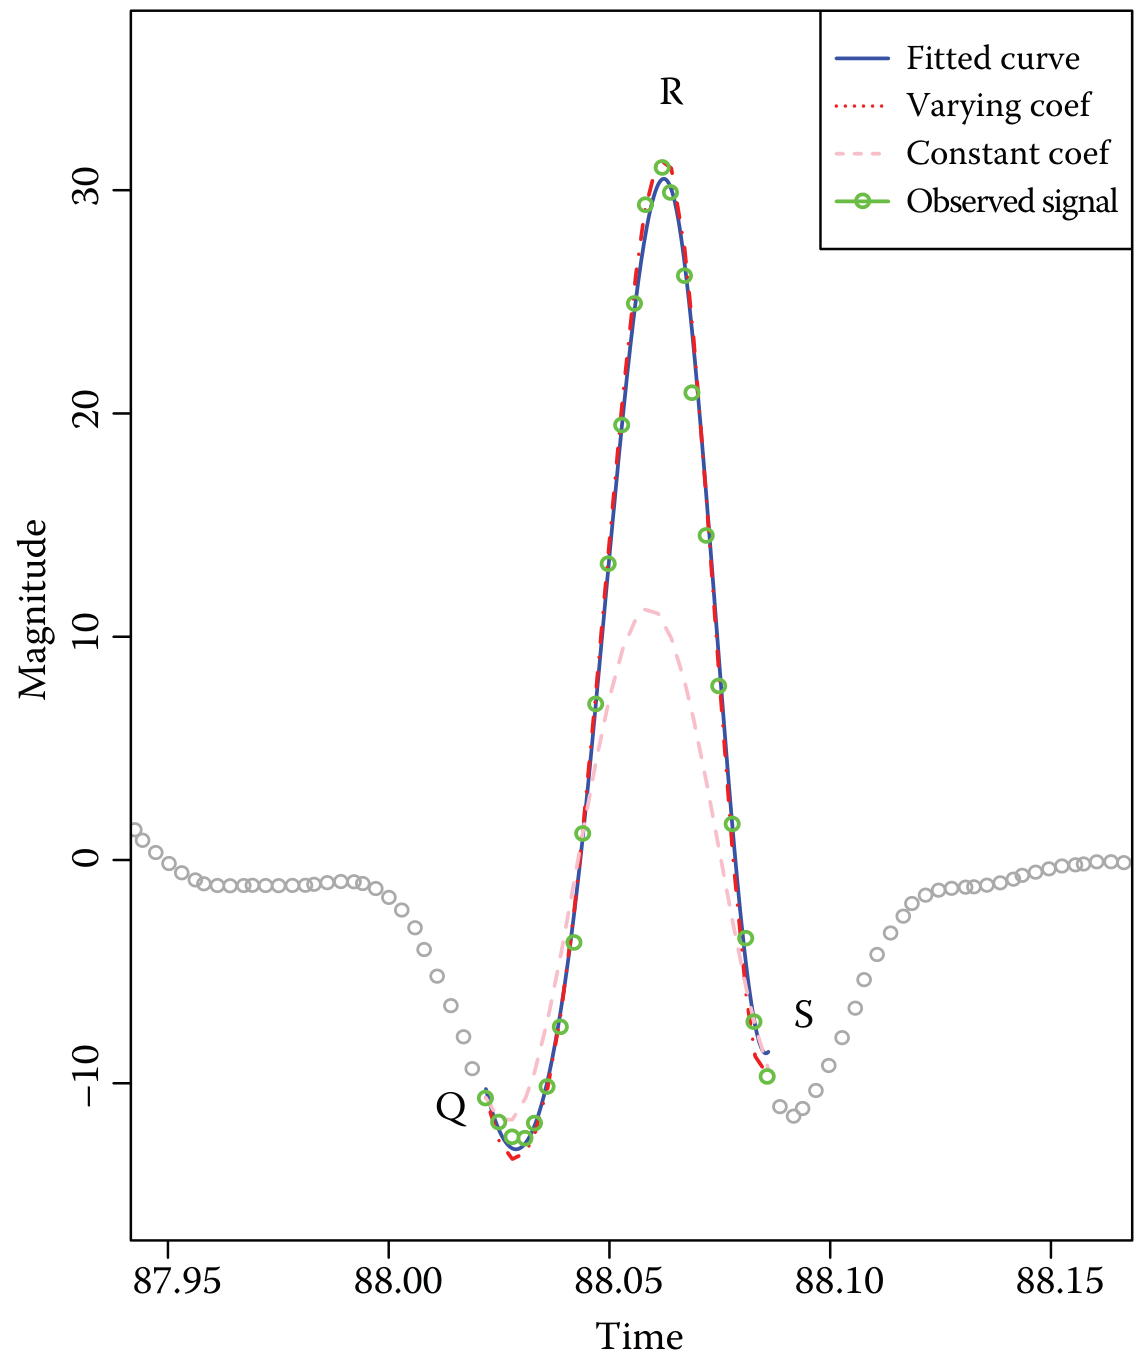
\includegraphics[width=10.5cm]{figures/ch03_fig03_data.png}};
\fill[white] (8.2895,10.3480) rectangle (10.3987,12.4941);
\fill[white] (5.4482,0.0817) rectangle (6.3258,0.4962);
\node[font=\scriptsize,rotate=0,inner sep=0] at (5.8870,0.2889) {时间};
\fill[white] (0.1063,6.1370) rectangle (0.5300,7.8634);
\node[font=\scriptsize,rotate=90,inner sep=0] at (0.3182,7.0002) {幅值};
\node[font=\scriptsize,rotate=0,inner sep=0] at (9.1469,12.0658) {拟合曲线};
\node[font=\scriptsize,rotate=0,inner sep=0] at (9.1909,11.6268) {时变系数};
\node[font=\scriptsize,rotate=0,inner sep=0] at (9.2775,11.1879) {常系数};
\node[font=\scriptsize,rotate=0,inner sep=0] at (9.3236,10.7489) {观测信号};
\end{tikzpicture}
\origfig{3}{二阶常微分方程拟合得到的曲线。}
\label{fig:ch03-03}
\end{figure}

\begin{figure}[htbp]
\centering
\begin{tikzpicture}[x=1cm,y=1cm]
\node[anchor=south west,inner sep=0] at (0,0) {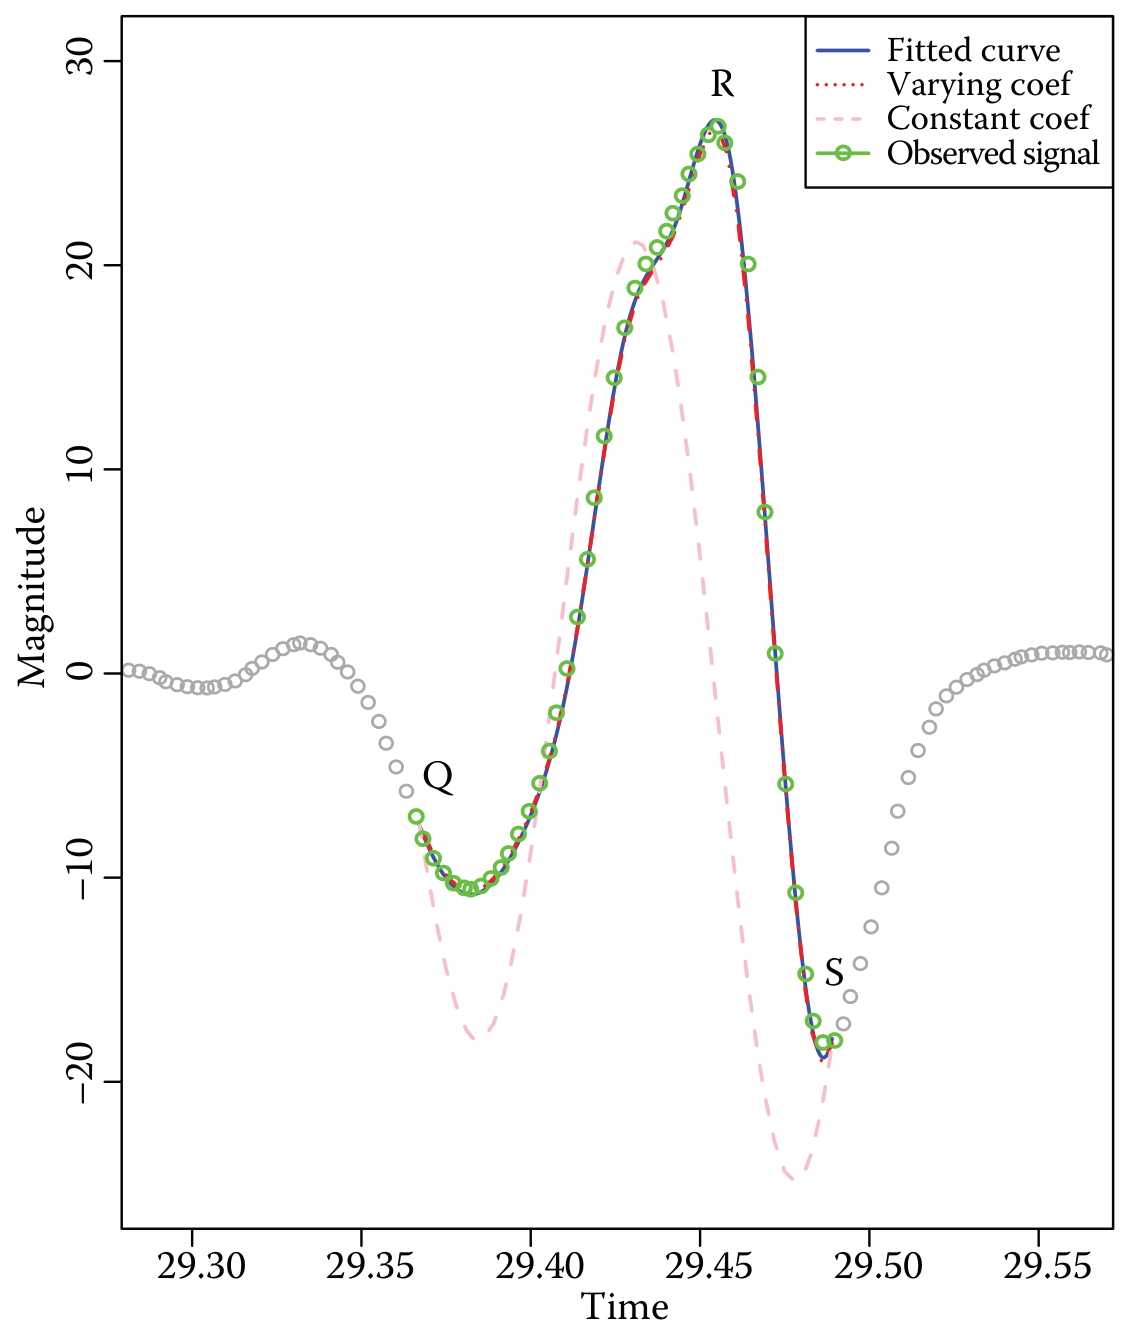
\includegraphics[width=10.5cm]{figures/ch03_fig04_data.png}};
\fill[white] (8.2460,10.7427) rectangle (10.3553,12.2827);
\fill[white] (5.3825,0.0329) rectangle (6.2718,0.4529);
\node[font=\scriptsize,rotate=0,inner sep=0] at (5.8272,0.2429) {时间};
\fill[white] (0.0991,6.0075) rectangle (0.5284,7.7569);
\node[font=\scriptsize,rotate=90,inner sep=0] at (0.3137,6.8822) {幅值};
\node[font=\scriptsize,rotate=0,inner sep=0] at (9.0889,11.9754) {拟合曲线};
\node[font=\scriptsize,rotate=0,inner sep=0] at (9.1335,11.6555) {时变系数};
\node[font=\scriptsize,rotate=0,inner sep=0] at (9.2214,11.3356) {常系数};
\node[font=\scriptsize,rotate=0,inner sep=0] at (9.2714,11.0158) {观测信号};
\end{tikzpicture}
\origfig{4}{时变二阶常微分方程对异常 QRS 波群的拟合曲线。}
\label{fig:ch03-04}
\end{figure}

\FloatBarrier

\bookdeepheading{paragraph}{3.1.3.3.2}{稳定性与瞬态响应分析}

常参数二阶 ODE 虽然只能近似观测信号曲线的形状，却能够很好地刻画 QRS 波群的动态行为。动态性质包括稳定性（stability）和瞬态响应（transient response），它们决定系统能否在各种随机内外扰动下维持功能与性能，以及系统如何响应环境变化。

生物系统最重要的动态性质是稳定性。如果一个动态系统在受到内部或外部扰动后，其状态变量返回或趋近原状态或平衡状态，就称该系统稳定（Kremling and Saez-Rodriguez 2007）。稳定性是系统本身的性质。判断动态系统稳定性的一种方法，是分析描述线性动态系统的高阶 ODE 的特征方程之特征值。如果所有特征值的实部均为负，系统稳定；如果所有特征值的实部均为正，系统不稳定。图3.3中正常 QRS 波群的二阶 ODE 系数为 $w_1=2.598$、$w_0=9394.2$，其特征值为 $\lambda_1=-1.30+96.9i$ 和 $\lambda_2=-1.30-96.9i$。图3.4中异常 QRS 波群的二阶 ODE 系数为 $w_1=-6.97$、$w_0=4535.9$，其特征值为 $\lambda_1=3.48+67.26i$ 和 $\lambda_2=3.48-67.26i$。可以清楚看到，正常 QRS 波群的二阶 ODE 所有特征值实部均为负，而异常 QRS 波群的所有特征值实部均为正。这说明正常 QRS 波群稳定，异常波群不稳定。在外部扰动发生之前，心脏动态系统维持稳态。根据环境扰动之后系统的动态行为，系统的稳态可能稳定，即返回初始状态；也可能不稳定，即离开初始平衡状态。出于任何实际目的，动态 QRS 波群都必须稳定。异常 QRS 波群背后的不稳定动态系统，会导致心脏活动不规则，甚至导致心力衰竭。

QRS 波群背后心脏系统的动态行为，编码在其状态随时间的演化之中。生物系统对内部和外部刺激扰动的响应，包含瞬态响应与稳态响应两部分。系统响应内外刺激扰动时，从初始状态过渡到最终状态的过程，称为瞬态响应。稳态响应则研究时间趋于无穷时的系统行为。对心脏系统进行瞬态响应分析，可以量化其动态特性，揭示心脏动态系统响应环境扰动的速度，以及最终达到目标稳态值的准确程度。还可以据此研究心脏动态系统的阻尼振荡行为和稳定性。

动态系统的瞬态响应依赖输入信号，不同信号会产生不同响应。实际中存在多种信号。为便于比较，考虑两种信号：（1）单位阶跃信号；（2）单位冲激信号。

QRS 波群背后心脏动态系统对单位阶跃和单位冲激输入信号的响应传递函数，分别为 $Y(s)=G(s)/S$ 和 $Y(s)=G(s)$，其中 $G(s)$ 为动态系统的传递函数。可以通过 Laplace 逆变换分析动态系统的瞬态响应。这里使用 MATLAB\textsuperscript{\textregistered} 进行瞬态响应分析（Ogata 1997）。图3.5和图3.6分别展示了正常与异常 QRS 波群所对应心脏系统的单位阶跃响应曲线，两者存在显著差异。正常与异常 QRS 波群都出现信号振荡；但是，正常 QRS 波群在单位阶跃扰动后很快达到稳态，而异常 QRS 波群的扰动响应高度振荡，始终无法达到稳态值。这表明，异常 QRS 波群对环境刺激的动态响应不规则。图3.7和图3.8分别展示了正常与异常 QRS 波群所对应心脏系统的单位冲激响应曲线，其模式与 QRS 波群的单位阶跃响应相似。

\begin{figure}[htbp]
\centering
\begin{tikzpicture}[x=1cm,y=1cm]
\node[anchor=south west,inner sep=0] at (0,0) {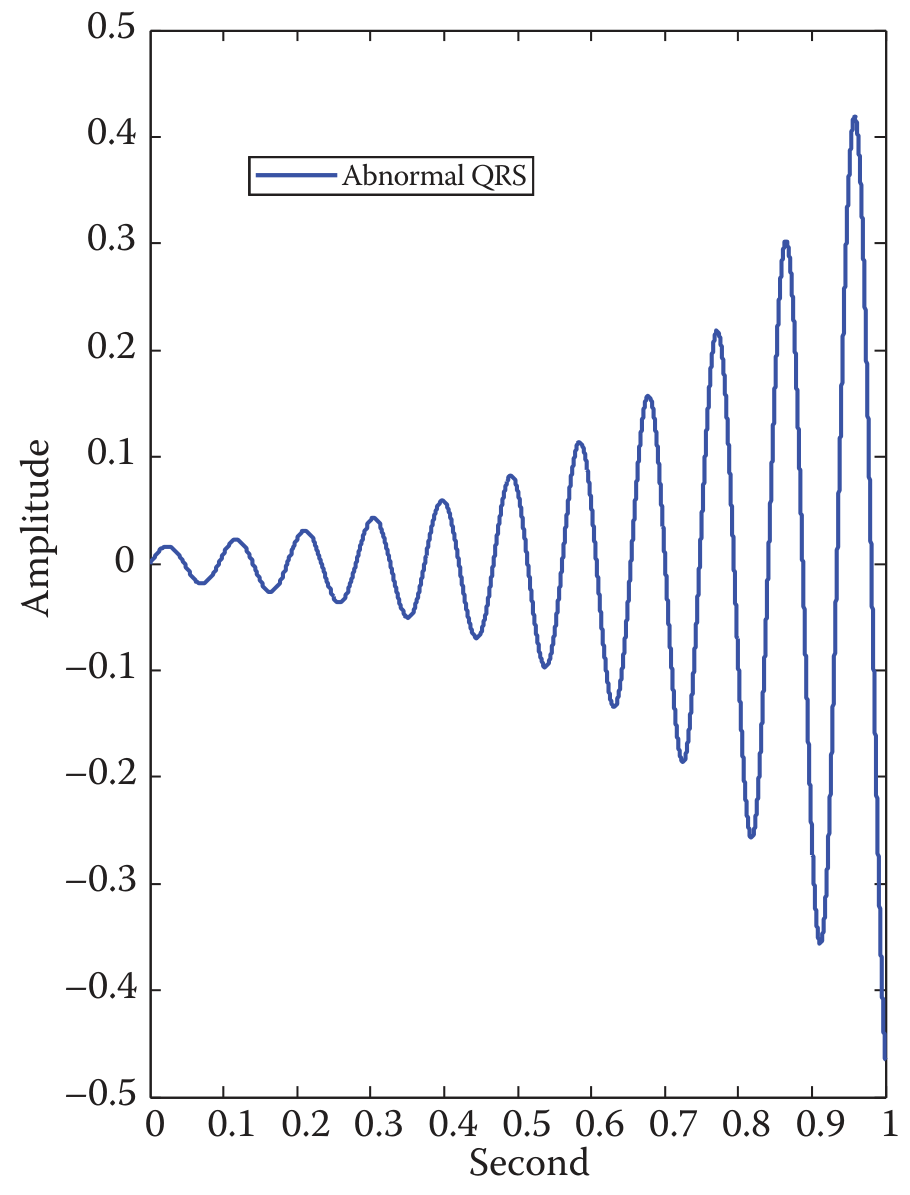
\includegraphics[width=9.0cm]{figures/ch03_fig05_data.png}};
\fill[white] (3.3626,9.9148) rectangle (5.2418,10.2412);
\fill[white] (4.6029,0.0749) rectangle (5.8648,0.5199);
\node[font=\scriptsize,rotate=0,inner sep=0] at (5.2339,0.2974) {时间（秒）};
\fill[white] (0.1459,5.6806) rectangle (0.6008,7.5043);
\node[font=\scriptsize,rotate=90,inner sep=0] at (0.3733,6.5924) {振幅};
\node[font=\scriptsize,rotate=0,inner sep=0] at (4.2946,10.0599) {异常 QRS};
\end{tikzpicture}
\origfig{5}{正常 QRS 波群所对应心脏系统的单位阶跃响应曲线。}
\label{fig:ch03-05}
\end{figure}

\begin{figure}[htbp]
\centering
\begin{tikzpicture}[x=1cm,y=1cm]
\node[anchor=south west,inner sep=0] at (0,0) {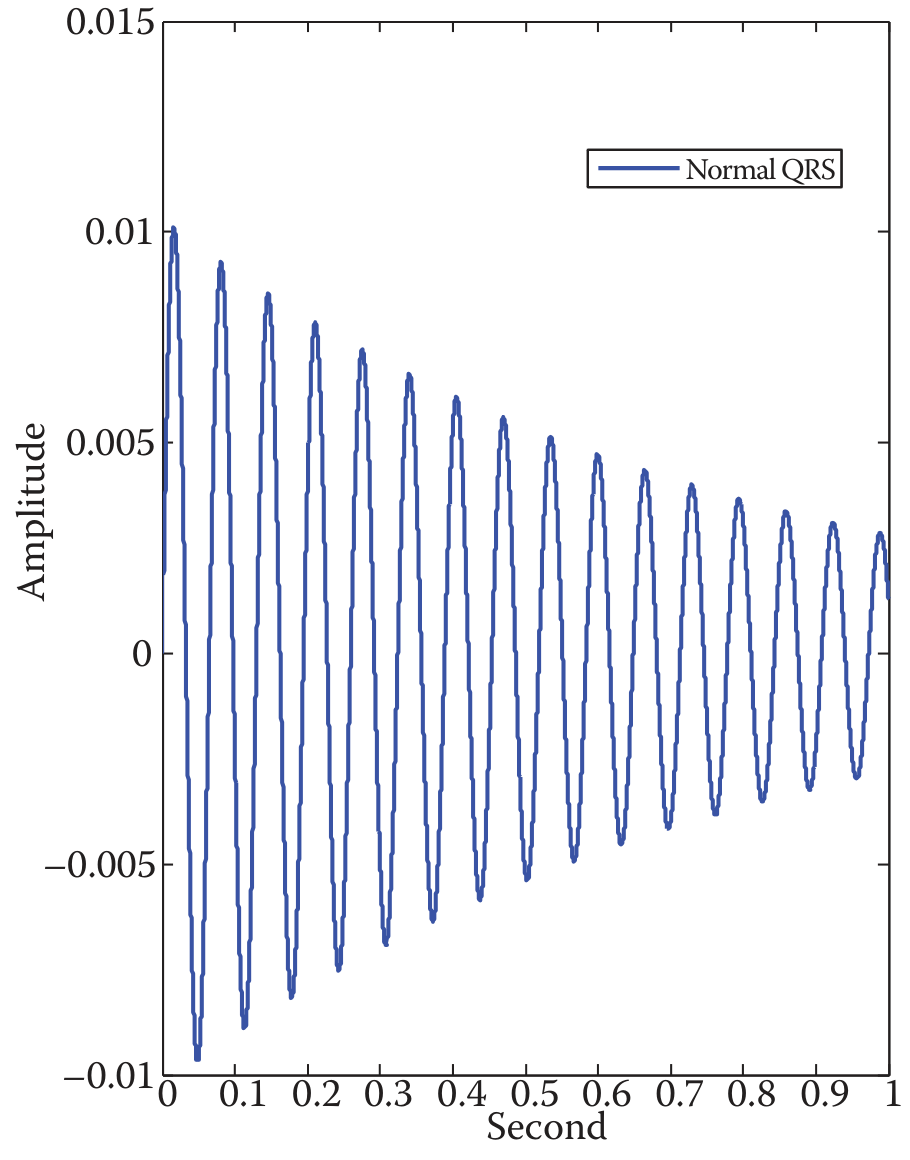
\includegraphics[width=9.0cm]{figures/ch03_fig06_data.png}};
\fill[white] (6.7747,9.6527) rectangle (8.2879,9.9692);
\fill[white] (4.7771,0.0876) rectangle (6.0391,0.5327);
\node[font=\scriptsize,rotate=0,inner sep=0] at (5.4081,0.3102) {时间（秒）};
\fill[white] (0.1122,5.4948) rectangle (0.5672,7.3185);
\node[font=\scriptsize,rotate=90,inner sep=0] at (0.3397,6.4066) {振幅};
\node[font=\scriptsize,rotate=0,inner sep=0] at (7.5230,9.7811) {正常 QRS};
\end{tikzpicture}
\origfig{6}{异常 QRS 波群所对应心脏系统的单位阶跃响应曲线。}
\label{fig:ch03-06}
\end{figure}

\begin{figure}[htbp]
\centering
\begin{tikzpicture}[x=1cm,y=1cm]
\node[anchor=south west,inner sep=0] at (0,0) {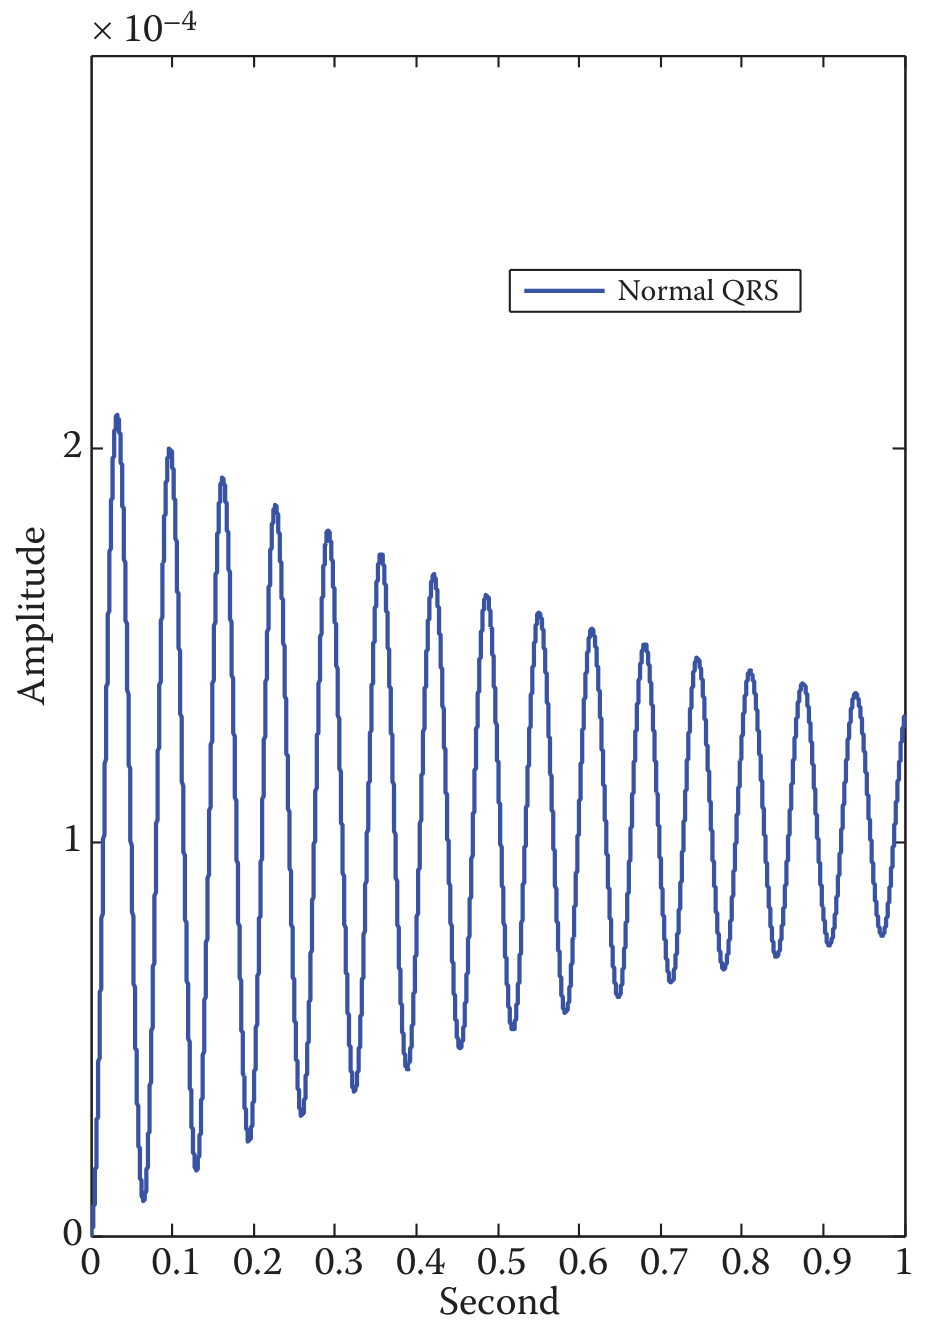
\includegraphics[width=9.0cm]{figures/ch03_fig07_data.png}};
\fill[white] (5.9838,9.9924) rectangle (7.7595,10.3427);
\fill[white] (4.2377,0.0854) rectangle (5.4792,0.5232);
\node[font=\scriptsize,rotate=0,inner sep=0] at (4.8585,0.3043) {时间（秒）};
\fill[white] (0.1094,6.0974) rectangle (0.5570,7.8916);
\node[font=\scriptsize,rotate=90,inner sep=0] at (0.3332,6.9945) {振幅};
\node[font=\scriptsize,rotate=0,inner sep=0] at (6.7949,10.1397) {正常 QRS};
\end{tikzpicture}
\origfig{7}{正常 QRS 波群所对应心脏系统的单位冲激响应曲线。}
\label{fig:ch03-07}
\end{figure}

\begin{figure}[htbp]
\centering
\begin{tikzpicture}[x=1cm,y=1cm]
\node[anchor=south west,inner sep=0] at (0,0) {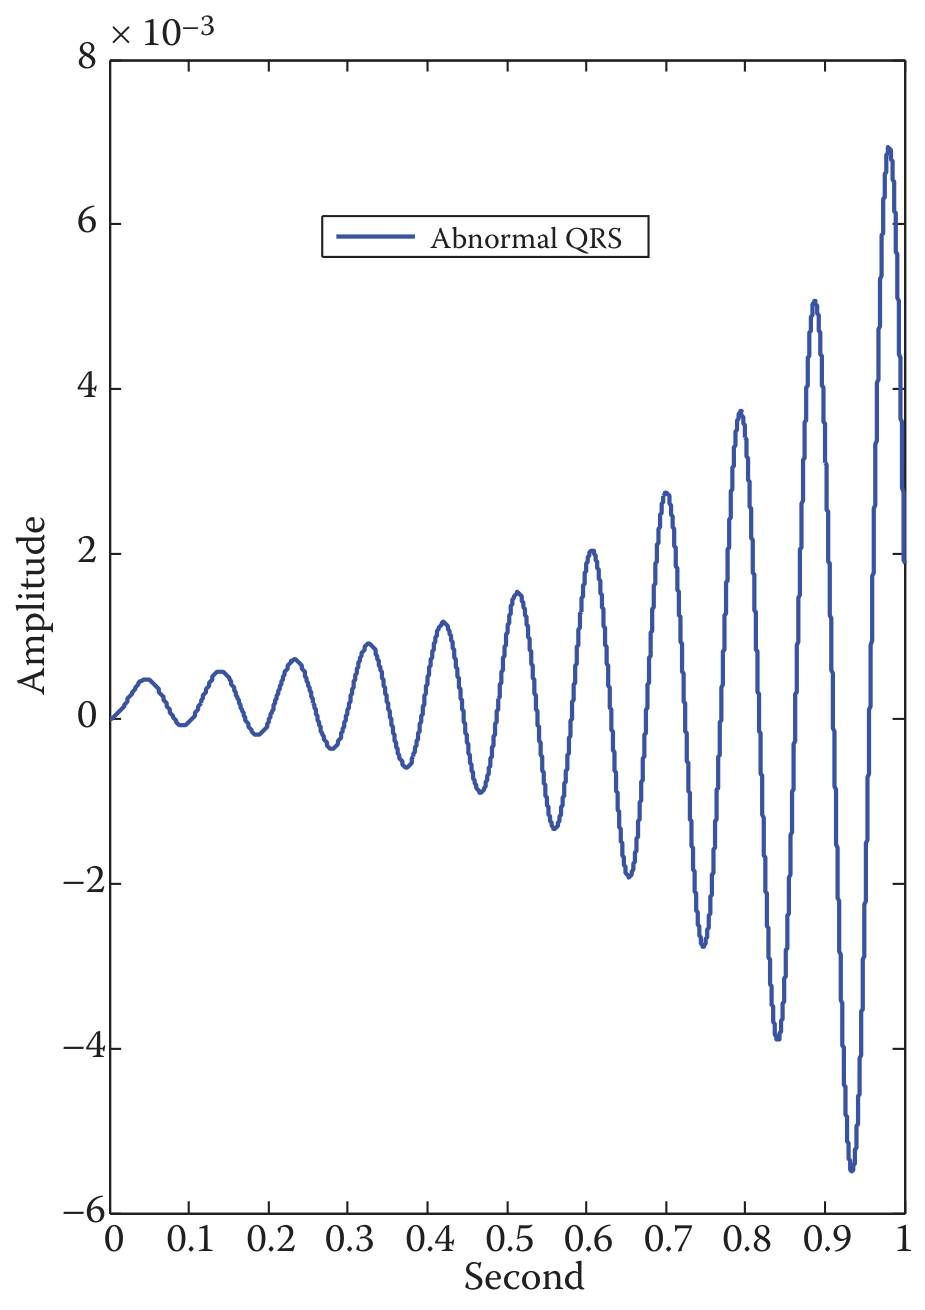
\includegraphics[width=9.0cm]{figures/ch03_fig08_data.png}};
\fill[white] (4.1692,10.2795) rectangle (6.2757,10.6103);
\fill[white] (4.4824,0.0841) rectangle (5.7239,0.5219);
\node[font=\scriptsize,rotate=0,inner sep=0] at (5.1031,0.3030) {时间（秒）};
\fill[white] (0.1067,5.9560) rectangle (0.5542,7.7501);
\node[font=\scriptsize,rotate=90,inner sep=0] at (0.3304,6.8530) {振幅};
\node[font=\scriptsize,rotate=0,inner sep=0] at (5.1206,10.4108) {异常 QRS};
\end{tikzpicture}
\origfig{8}{异常 QRS 波群所对应心脏系统的单位冲激响应曲线。}
\label{fig:ch03-08}
\end{figure}

\FloatBarrier

\bookdeepheading{paragraph}{3.1.3.3.3}{动态系统信号的分类}

前面的研究充分表明，二阶 ODE 能够有效捕捉 QRS 波群的动态特征。下面评价将二阶 ODE 参数用于 QRS 波群分类的性能。使用三个指标评价分类性能：灵敏度、特异度与准确率。灵敏度定义为真实异常信号被正确分类为异常的百分比；特异度定义为真实正常信号被正确分类为正常的百分比；分类准确率定义为正常及异常信号被正确分类的百分比。我们使用 MIT/BIH 数据库中的19条心电记录（Ravier et al. 2007），将二阶 ODE 参数作为 QRS 波群特征，输入支持向量机（support vector machine，SVM）（Chang and Lin 2011）进行分类。同时，将结果与 Ravier et al.（2007）使用的神经网络分类器比较。对于二阶 ODE 的时变参数，将参数函数 $w_0(t)$ 和 $w_1(t)$ 的函数主成分得分（Ramsay and Silverman 2005）作为 SVM 特征。具体而言，将 QRS 波群信号按 Fourier 级数展开，将 Fourier 展开系数作为多层神经网络（neural network，NN）的特征；该网络含16个输入节点、隐藏层的4个神经元，以及1个输出神经元。对于常参数 ODE 和时变参数 ODE，还将 R 点高度与 QRS 波群宽度作为特征。

分类结果汇总于表3.1。其中，ODE 表示常参数常微分方程，ODET 表示时变参数常微分方程，NN 表示神经网络。表3.1的结果呈现出以下特征。第一，多数情况下，常参数 ODE 的准确率最高。第二，一个令人意外的现象是：时变参数 ODE 的解轨迹对 QRS 波群观测曲线的逼近效果，远好于常参数 ODE；然而，在许多情况下，其 QRS 波群分类性能却不及常参数 ODE。第三，当正常与异常 QRS 波群的样本量极不平衡时（记录51、100、101、202），三个分类器的灵敏度或特异度均明显不准确，因为训练样本没有提供足够信息来区分正常与异常 QRS 波群。一般而言，正常 QRS 波群的样本数远大于异常波群时，分类特异度较高；反之，异常波群样本数更多时，可以获得较高的灵敏度。第四，正常与异常 QRS 波群样本量平衡时，灵敏度和特异度均可达到较高水平。

\begin{table}[p]
\centering
\origtable{1}{常系数常微分方程、时变参数常微分方程与神经网络对 QRS 波群的分类准确率。}
\label{tab:ch03-01}
\begingroup
\footnotesize
\setlength{\tabcolsep}{3.6pt}
\begin{tabular}{rrr*{9}{r}}
\toprule
\multirow{2}{*}{文件号}&\multirow{2}{*}{\shortstack{正常QRS\\数量}}&\multirow{2}{*}{\shortstack{异常QRS\\数量}}&
\multicolumn{3}{c}{灵敏度}&\multicolumn{3}{c}{特异度}&\multicolumn{3}{c}{准确率}\\
\cmidrule(lr){4-6}\cmidrule(lr){7-9}\cmidrule(lr){10-12}
&&&ODE&ODET&NN&ODE&ODET&NN&ODE&ODET&NN\\
\midrule
100 & 2233 & 34 & 0.059 & 0.118 & 0.235 & 0.999 & 0.999 & 0.995 & 0.985 & 0.985 & 0.983\\
101 & 1851 & 8 & 0.250 & 0.000 & 0.167 & 1.000 & 1.000 & 1.000 & 0.997 & 0.996 & 0.997\\
102 & 99 & 2082 & 1.000 & 1.000 & 0.998 & 0.980 & 0.909 & 0.788 & 0.999 & 0.996 & 0.988\\
104 & 163 & 2060 & 0.969 & 0.992 & 0.983 & 0.699 & 0.675 & 0.783 & 0.950 & 0.969 & 0.964\\
105 & 2484 & 110 & 0.745 & 0.273 & 0.622 & 0.988 & 1.000 & 0.996 & 0.978 & 0.969 & 0.990\\
106 & 1500 & 511 & 0.990 & 0.990 & 0.939 & 0.999 & 0.970 & 0.978 & 0.997 & 0.975 & 0.968\\
119 & 1539 & 444 & 1.000 & 1.000 & 0.995 & 1.000 & 0.995 & 0.992 & 1.000 & 0.996 & 0.993\\
200 & 1736 & 847 & 0.919 & 0.939 & 0.867 & 0.997 & 0.929 & 0.963 & 0.971 & 0.932 & 0.931\\
201 & 1604 & 272 & 0.853 & 0.673 & 0.747 & 0.999 & 0.993 & 0.991 & 0.978 & 0.946 & 0.956\\
202 & 2044 & 69 & 0.391 & 0.188 & 0.306 & 0.999 & 0.997 & 0.991 & 0.979 & 0.971 & 0.971\\
205 & 2564 & 83 & 0.867 & 0.084 & 0.790 & 1.000 & 1.000 & 0.995 & 0.995 & 0.971 & 0.988\\
208 & 1573 & 1356 & 0.973 & 0.982 & 0.945 & 0.987 & 0.941 & 0.960 & 0.980 & 0.960 & 0.953\\
209 & 2616 & 384 & 0.444 & 0.447 & 0.482 & 0.981 & 0.978 & 0.976 & 0.912 & 0.910 & 0.912\\
210 & 2410 & 212 & 0.882 & 0.269 & 0.770 & 0.995 & 0.999 & 0.954 & 0.986 & 0.940 & 0.940\\
212 & 919 & 1824 & 0.967 & 0.971 & 0.958 & 0.984 & 0.928 & 0.958 & 0.973 & 0.957 & 0.958\\
213 & 2634 & 609 & 0.849 & 0.875 & 0.863 & 0.995 & 0.983 & 0.987 & 0.968 & 0.963 & 0.964\\
215 & 2412 & 120 & 0.958 & 0.196 & 0.800 & 0.997 & 0.904 & 0.986 & 0.995 & 0.705 & 0.979\\
217 & 242 & 1959 & 0.995 & 0.993 & 0.987 & 0.946 & 0.946 & 0.964 & 0.990 & 0.988 & 0.984\\
219 & 1539 & 51 & 0.824 & 0.278 & 0.667 & 1.000 & 0.862 & 0.994 & 0.994 & 0.697 & 0.986\\
\bottomrule
\end{tabular}
\endgroup
\end{table}

\FloatBarrier
